\documentclass{article}
\usepackage{graphicx}
\usepackage{amsmath}
\usepackage{pgfplots}
\usepackage{physics}
\usepackage{cancel}
\usepackage{enumitem}
\usepackage{txfonts}

\pgfplotsset{compat=1.18}

\newcommand{\Eth}{E_{\text{th}}}

\usepackage[a4paper, top=1cm, bottom=2cm, left=2cm, right=2cm, includehead, includefoot]{geometry}

\begin{document}

\noindent
Physics 4A - Classical Mechanics \hfill Prof. Roger King

\noindent\rule{\textwidth}{0.4pt}

\begin{center}
    \textbf{\LARGE Homework 11} \\
    \vspace{12pt}
    \large Aaron W. Tarajos \\
    \textit{\today}
\end{center}

\noindent\rule{\textwidth}{0.4pt}

\section*{Problem 1}
A neutron at rest decays into a proton, an electron, and a neutrino. If the proton's momentum
is $3.00 \times 10^{-24}$ kg m/s in the direction 37$^\circ$ N of E and the electron's momentum is $4.00 \times 10^{-24}$ kg
m/s in the direction 53$^\circ$ S of W, what is the momentum of the neutrino?

\subsection*{Solution}
Since the neutrino is at rest we just need to find the value of the neutrino momentum vector such that the resultant of all three particles is zero.
\begin{align*}
	0 &= \vec{p}_\text{p} + \vec{p}_\text{e} + \vec{p}_\text{n} \\
	- \vec{p}_\text{p} &= \vec{p}_\text{e} + \vec{p}_\text{n} \\
	- \vec{p}_\text{p} &= 3.00 \times 10^{-24}\cos(37)\ \vu{i} + 3.00 \times 10^{-24}\sin(37)\ \vu{j} \\
							   &+ 4.00 \times 10^{-24}\cos(233)\ \vu{i} + 4.00 \times 10^{-24}\sin(233) \ \vu{j} \\
	- \vec{p}_\text{p} &= -1.135\times10^{-26}\ \vu{i} -1.389\times10^{-24}\ \vu{j} \\
	\vec{p}_\text{p}   &= \boxed{1.135\times10^{-26}\ \vu{i} + 1.389\times10^{-24}\ \vu{j} \ \text{kg}\ \text{m}/\text{s}}
\end{align*}


\section*{Problem 2}
A 60.0-g tennis ball strikes the ground at 25.0 m/s at 40$^\circ$ to the horizontal. It bounces off at
20.0 m/s at 30$^\circ$ to the horizontal. (a) Find the impulse exerted on the ball. (b) If the collision
lasted 5.00 ms, find the average force exerted on the ball by the court.

\begin{figure}[ht]
    \centering
    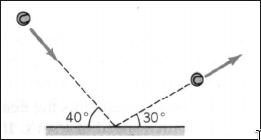
\includegraphics[scale=0.5]{drawing-1.png}
\end{figure}

\subsection*{Solution}
\subsubsection*{Part a:}
The impulse is given by;
\[
	\vec{J} = \Delta \vec{p}
\]
Therefore;
\begin{align*}
	\vec{J} &= \left[ (60.0)(20)\cos(30)\ - (60)(25)\cos(-40) \right] \vu {i} + \left[ (60)(20)\sin(30)  - (60)(25)\sin(-40)\right] \vu{j} \\
		&= \boxed{-109.836\ \vu i + 1564.181\ \vu j \ \text{g}\ \text{m}/\text{s}}
\end{align*}

\subsubsection*{Part b:}
The average force is equal to the change in impluse over time;
\[
	\vec{F}_\text{avg} = \frac{-109.836\ \vu i 156.181\ \vu j}{0.05} = \boxed{-2196.724\ \vu{i} -31\ 283.628\ \vu{j} \ \text{g}\ \text{m}/\text{s}^2}
\]

\section*{Problem 3}
A 1000-kg Subaru at rest at a stoplight is struck from the rear by a 1400-kg Pontiac. They
couple together and leave skid marks 4.25 m long. The coefficient of kinetic friction is 0.6. (a)
What was their common speed just after the collision? (b) What was the speed of the Pontiac just
prior to the collision?

\section*{Solution}
\subsubsection*{Part a:}
The work done by friction is $W = \vec{F}_n \cdot d$ while work is also equal to $\Delta K$ so we have;
\begin{align*}
	W &= \Delta K \\
	\vec{F}_n \cdot d &= K_f - K_i \\
	(\mu_k)(m_1 + m_2)g \cos(\theta)d &= 0 - \frac{1}{2} (m_1 + m_2)v^2 \\
	v^2 &= -2g \mu_k \cos(\theta) d \\
	v &= \sqrt{-2g \mu_k \cos(\theta) d} \\
	v &= \sqrt{(-2)(9.81)(0.60)\cos(180)(4.25)} \\
	v &= \boxed{7.07\ \text{m}/\text{s}}
\end{align*}

\subsubsection*{Part b:}
Using conservation of momentum we can say that;
\[
	m_1 v_{1i} + m_2 v_{2i} = m_1 v_{1f} + m_2 v_{2f}
\]
and then solve for $v_{2i}$
\begin{align*}
	v_{2i} &= \frac{m_1 v_{1f} + m_2 v_{2f} - m_1 v_{1i}}{m_2} \\
	       &= \frac{(1000)(7.07) + (1400)(7.07) - (1000)(0)}{1400} \\
	       &= \boxed {12.12 \ \text{m}/\text{s}}
\end{align*}

\section*{Problem 4}
Two particles with masses $m_1$ and $m_2$ travel toward each other with velocities $v_{1,i}$ and $v_{2,i}$.
They collide and stick together. Show that the loss in kinetic energy is
\[
	\frac{m_1m_2(v_{1,i} - v_{2,i})^2}{2(m_1 + m_2)}
\]

\subsection*{Solution}
The initial kinetic energy is
\[
	K_i = \frac{1}{2}m_1v_{1,i}^2 + \frac{1}{2}m_2v_{2,i}^2
\]
and the final kinetic energy is
\[
	K_f = \frac{1}{2}(m_1 + m_2)v_f^2
\]
We also know that $v_f$ from the conservation of momentum is given by;
\[
	v_f = \frac{m_1v_{1,i}-m_2v_{2,i}}{m_1 + m_2}
\]
and so we have
\begin{align*}
	\Delta K &= \frac{1}{2} m_1 v_{1,i}^2 + \frac{1}{2} m_2 v_{2,i}^2 - \frac{1}{2} (m_1 + m_2) v_f^2 \\
		 &= \frac{1}{2} \left[ m_1 v_{1,i}^2 + m_2 v_{2,i}^2 - \frac{(m_1 v_{1,i} + m_2 v_{2,i})^2}{m_1 + m_2} \right] \\
		 &= \frac{1}{2} \left[ \frac{(m_1 + m_2) m_1 v_{1,i}^2 + m_2 v_{2,i}^2 - (m_1 v_{1,i} + m_2 v_{2,i})^2}{m_1 + m_2} \right] \\
		 &= \frac{m_1m_2(v_{1,i - v_{2,i}})^2}{2(m_1 + m_2)}
\end{align*}

\section*{Problem 5}
A projectile of mass 0.25 kg moving at 24.0 m/s collides with and sticks to a 1.75-kg block
that is connected to a spring for which k = 40.0 N/m, as in the figure below. The block is
initially on a frictionless part of a horizontal surface but starts to slide on a rough section
immediately after the collision. If the maximum compression of the spring is 0.5 m, what is the
force of friction on the block?

\begin{figure}[ht]
    \centering
    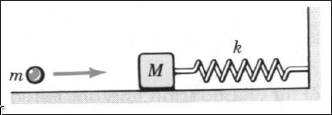
\includegraphics[scale=0.5]{drawing-2.png}
\end{figure}

\subsection*{Solution}
Using the conservation of momentum to find velocity at the collision;
\[
	v_f = \frac{m v_i}{m+M}
\]
then the kinetic energy after the collision is converted into potential energy and work done against friction;
\begin{align*}
	\frac{1}{2}(m+M)\left(\frac{m v_i}{m+M}\right)^2 &= \frac{1}{2}kx^2 + \vec{F}_k x \\
	\vec{F}_k &= \left(\frac{1}{2}(m+M)\left(\frac{m v_i}{m+M}\right)^2 - \frac{1}{2}kx^2\right) \cdot \frac{1}{x}\\
	\vec{F}_k &= \left(\frac{1}{2}(0.25+1.75)\left(\frac{0.25 24.0}{0.25+1.75}\right)^2 - \frac{1}{2}(40.0)(0.5)^2 \right) \cdot \frac{1}{0.5} \\
		  &= \boxed{8.0 \ \text{N}}
\end{align*}

\section*{Problem 6}
From the $F$ versus $t$ curve shown below, find: (a) the impulse; (b) the average force.


\begin{figure}[ht]
    \centering
    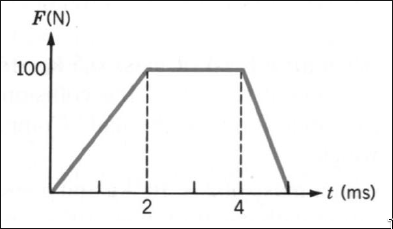
\includegraphics[scale=0.5]{drawing-3.png}
\end{figure}

\subsection*{Solution}
\subsubsection*{Part a:}
The impulse is
\[
	\vec{J} = \int \vec{F} dt
\]
for the given graph that is
\[
	\vec{J} = \frac{1}{2}(2)(100) + (100)(2) + \frac{1}{2}(100)(1) = \boxed{350 \ \text{N} \cdot \text{ms}}
\]

\subsubsection*{Part b:}
The average force is given by;

\[
	\frac{\vec{J}}{\Delta t} = \frac{350}{5} = \boxed{70\ \text{N}}
\]

\section*{Problem 7}
A nucleus of radioactive radium ($^{226}$Ra), initially at rest, decays into a radon nucleus ($^{222}$Rn)
and an $\alpha$-particle (a $^4$He nucleus). If the kinetic energy of the $\alpha$-particle is 6.72 $\times$ 10 $^{-13}$ J,
what is (a) the recoil speed of the radon nucleus, and (b) its kinetic energy? The superscripts
indicate, roughly, the mass of each nucleus in unified mass units (u), where 1 u = 1.66 $\times$
10$^{-27}$ kg.

\subsection*{Solution}
\subsubsection*{Part a:}
Using conservation of momentum and solving for $v_\text{Rn}$;
\begin{align*}
	m_\alpha v_\alpha &= -m_\text{Rn}v_\text{Rn} \\
	v_\text{Rn} &= \frac{m_\alpha v_\alpha}{-m_\text{Rn}} \\
\end{align*}
Then using kinetic energy to solve for velocity;
\begin{align*}
	K_\alpha &= \frac{1}{2}m_\alpha v_\alpha^2 \\
	v_\alpha &= \sqrt{\frac{2 K_\alpha}{m_\alpha}} \\
	v_\alpha &= \sqrt{\frac{2 K_\alpha}{m_\alpha}} \\
\end{align*}
Givng us the equation;
\begin{align*}
	v_\text{Rn} &= \frac{(4 \times 1.66 \times 10^{-27}) \sqrt{\frac{2 \times 6.72 \times 10^{-13}}{4 \times 1.66 \times 10^{-27}}}}{222 \times 1.66 \times 10^{-27}} \\
	v_\text{Rn} &= \boxed{2.563 \times 10^{5} \text{m}/\text{s}}
\end{align*}

\subsubsection*{Part b:}
The kinetic energy is given by
\[
	K = \frac{1}{2}mv^2
\]
so we have
\[
	K = \frac{1}{2} \cdot 222 \times 1.66 \times 10^{-27} \times (2.56 \times 10^5)^2 = \boxed{1.21 \times 10^{-14}\ \text{J}}
\]

\section*{Problem 8}
A projectile of mass $m$ = 200 g strikes a stationary block of mass $M$ = 1.30 kg from below
with speed $u$ = 30.0 m/s as shown in the figure below. The projectile embeds in the block. (a)
To what height does the block rise? (b) What is the loss in kinetic energy due to the collision?

\begin{figure}[ht]
    \centering
    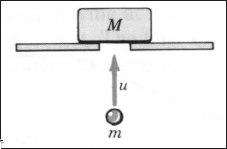
\includegraphics[scale=0.5]{drawing-4.png}
\end{figure}

\subsection*{Solution}
\subsubsection*{Part a:}
Using the conservation of momentum to find the velocity after the collision;
\[
	v = \frac{mu}{m+M}
\]
Then the height is given by
\[
	(m+M)gh = \frac{1}{2}(m+M)v^2
\]
so we have

\[
	h = \frac{v^2}{2g} = \frac{\left( \frac{mu}{m+M} \right)^2}{2g} = \frac{\left( \frac{200 \cdot 30.0}{1500} \right)^2}{2 \cdot 9.81} = \boxed{0.815 \ \text{m}}
\]

\subsubsection*{Part b:}
\[
	\Delta K = \frac{1}{2}(1500)(4.0)^2 - \frac{1}{2}(200)(30.0)^2 = \boxed{-78.0\ \text{J}}
\]

\end{document}
